\documentclass[11pt,a4paper]{article}

%----- ENHANCED TYPOGRAPHY -----
\usepackage[utf8]{inputenc}
\usepackage[T1]{fontenc}
\usepackage{lmodern}        % clean vector font
\usepackage{microtype}      % better justification & kerning
\usepackage{palatino} 
\usepackage{braket}   
\usepackage{mathtools}  % in the preamble
\usepackage{bbm}

%----- PAGE LAYOUT -----
\usepackage{geometry}
\geometry{top=1in, bottom=1in, left=1in, right=1in}
\usepackage{setspace}
\onehalfspacing  % 1.5 line spacing

%----- FANCY HEADERS & FOOTERS -----
\usepackage{fancyhdr}
\pagestyle{fancy}
\fancyhf{}
% page number outside, header text inside

\fancyhead[LO]{\small \rightmark}
\fancyhead[RO]{\small \leftmark}
\renewcommand{\headrulewidth}{0.4pt}
\renewcommand{\footrulewidth}{0pt}

% make sections feed into \leftmark/\rightmark
\renewcommand{\sectionmark}[1]{\markboth{#1}{}}
\renewcommand{\subsectionmark}[1]{\markright{#1}}

%----- SECTION NUMBERING & TOC DEPTH -----
\setcounter{secnumdepth}{3}  % number down to \subsubsection
\setcounter{tocdepth}{2}     % show ToC down to \subsection

%----- AMS MATH & THEOREM STYLES -----
\usepackage{amsmath,amssymb,mathtools}
\usepackage{amsthm}

% definitions, examples, remarks upright
\theoremstyle{definition}
\newtheorem{definition}{Definition}[section]
\newtheorem{example}[definition]{Example}
\newtheorem{remark}[definition]{Remark}

% theorems, lemmas, corollaries italic
\theoremstyle{plain}
\newtheorem{theorem}[definition]{Theorem}
\newtheorem{lemma}[definition]{Lemma}
\newtheorem{proposition}[definition]{Proposition}
\newtheorem{corollary}[definition]{Corollary}

% unnumbered proof environment
\theoremstyle{remark}

%----- OTHER PACKAGES -----
\usepackage{graphicx}
\usepackage{tikz}
\usetikzlibrary{arrows.meta,positioning}
\usetikzlibrary{calc, matrix, decorations.pathreplacing, positioning}
\usepackage{tikz-cd}
\usepackage{hyperref}
\hypersetup{colorlinks,
linkcolor=blue, citecolor=purple, urlcolor=teal}
\usepackage{enumitem}
\setlist[itemize]{nosep, left=1.5em}
\usepackage{booktabs}
\usepackage{listings}
\lstset{
basicstyle=\ttfamily\small,
numbers=left,
numbersep=5pt,
frame=single,
breaklines=true
}
\usepackage{xcolor}
\definecolor{shade}{HTML}{F5F5F5}
\usepackage{float}
%----- CUSTOM MACROS -----
\newcommand{\F}{\mathbb{F}}
\newcommand{\code}[1]{\texttt{#1}}
\newcommand{\dist}[2]{d\bigl(#1,#2\bigr)}
\newcommand{\R}{\mathbb{R}}
\newcommand{\Z}{\mathbb{Z}}
\newcommand{\N}{\mathbb{N}} 
\newcommand{\Q}{\mathbb{Q}} 
\newcommand{\C}{\mathbb{C}}
\renewcommand{\set}[1]{\left\{ #1 \right\}}
\newcommand{\angles}[1]{\langle #1 \rangle}
\newcommand{\abs}[1]{\lvert #1 \rvert}
\newcommand{\norm}[1]{\lVert #1 \rVert}
\newcommand{\1}{\mathbbm{1}}

% \usepackage{mathtools} 
% \DeclarePairedDelimiter{\angles}{\langle}{\rangle} 
% \DeclarePairedDelimiter{\braces}{\left\{}{\right\}} 
% \DeclarePairedDelimiter{\abs}{\lvert}{\rvert} 
% \DeclarePairedDelimiter{\norm}{\lVert}{\rVert}

%----- TITLE METADATA -----
\title{\LARGE\bfseries Algebraic Topology}
\author{Georges Khater \\ \small American University of Beirut, Math 314}
\date{\today}

%===============================================
\begin{document}
\maketitle
\tableofcontents
\bigskip

\section{Bases of the Fundamental Group}

\subsection{Homotopy equivalence.}
\begin{definition}
    Let $X$ be a topological space $f, g \colon X \to Y$ then we say that $f$ is \emph{homotopic} to $g$ 
    if there is a function $H \colon X \times I \to Y$ (called a homotopy) such that 
    $$H(x, 0) = f(x), \quad H(x, 1) = g(x)$$
\end{definition}

\begin{proposition}
    Homotopy is an equivalence relation. 
\end{proposition}

\begin{lemma}[Gluing Lemma]
    Suppose that $X = A \cup B$ with $A, B$ closed and take $f_1 \colon A \to Y$, $f_2 \colon B \to Y$. 
    s.t $f_1 (x) = f_2(x)$ for all $x \in A \cap B$. Then 
    $$f_3 \colon X \to Y, \quad f_3(x) = \begin{cases}
        f_1(x) \quad &\text{if $x \in A$} \\
        f_2(x) \quad &\text{if $x \in B$}
    \end{cases}$$
    is continuous.   
\end{lemma}

\begin{proof}
    Let $C$ be a closed set in $Y$, then 
    \begin{align*}
        f_3^{-1}(C) &= f_3^{-1}(C) \cap (A \cup B) \\
        &= \left(f_3^{-1}(C) \cap A\right) \cup \left( f_3^{-1} \cap B \right) \\
        &= f_1^{-1} (C) \cup f_2^{-1}(C)   
    \end{align*}
    which is closed in $X$.
\end{proof}

\begin{example}
    Any two function into $\R^n$ (convex set, start shaped set) are homotopic.

    Indeed, take two such $f(x), g(x)$ then let 
    $$H \colon X \times Y \to \R^n, \quad H(x, t) = (1-t) f(x) + t g(x)$$
    Note: we call this \emph{the straight line homotopy}. 
\end{example}

\paragraph{Relative Homotopy}
\begin{definition}
    Let $f,  g \colon X \to Y$ with $A \subseteq X$ and $f_{|A} = g_{|A}$ then 
    we say that $f$ is homotopic to $g$ relative to $A$ if there exists a homotopy $H \colon X \times I \to Y$ between $f$ and $g$ 
    $$H(x, t) = f(x) = g(x) \quad \forall t \in I, \ \forall x \in A$$ 
\end{definition}

\begin{remark}
    Homotopy is a special kind of relative  homotopy (for $A = \varnothing$). 
\end{remark}

\begin{proposition}
    Relative homotopy is an equivalence relation.
\end{proposition}

\begin{definition}
    Let $X$ a topological space and let $x_1, x_2 \in X$ then a path in $X$ going from $x_1$ to $x_2$ is a 
    function $\gamma \colon I \to X$ s.t 
    $$\gamma (0) = x_1, \quad \gamma(1) = x_2$$
\end{definition}

\begin{definition}
    Suppose that $\gamma_1$ and $\gamma_2$ are two paths in $X$ whose start point and end point coincide, then 
    we say that $\gamma_1$ is path homotopic to $\gamma_2$ if $\gamma_1$ is homotopic to $\gamma_2$ relative to $\set{0,1}$.

    Intuitively this means that we can deform $\gamma_1$ into $\gamma_2$ without moving the endpoints.
    i.e $H \colon I \times I \to X$ s.t 
    $$H (s,t) = \begin{cases}
        \gamma_1(s) \quad &\text{if } t = 0 \\
        \gamma_2(s) \quad &\text{if } t = 1 \\
        \gamma_1(0) = \gamma_2 (0) \quad &\text{if } s = 0 \\
        \gamma_1(1) = \gamma_2(1) \quad&\text{if } s = 1
    \end{cases}$$
\end{definition}

\begin{corollary}
    Path homotopy is an equivalence relation.
\end{corollary}

\begin{definition}
    $\gamma_1, \gamma_2 \colon I \to X$ with 
    $$\gamma_1(1) = \gamma_2(0)$$
    we define the \emph{product} of these paths to be the path $\gamma_1 \cdot \gamma_2$ given by 
    $$\gamma_1 \cdot \gamma_2 (s) = \begin{cases}
        \gamma(2s) \quad &\text{if } 0 \leq s \leq 1/2 \\
        \gamma(2s - 1) \quad &\text{if } 1/2 \leq s \leq 1
    \end{cases}$$
    Note that this is continuous by the Gluing Lemma.
\end{definition}

\begin{proposition}
    Path multiplication is compatible with path homotopy; i.e if 
    $$\gamma_1 \sim \gamma_1', \quad \gamma_2 \sim \gamma_2'$$
    then 
    $$\gamma_1 \cdot \gamma_2 \sim \gamma_1' \sim \gamma_2'$$
\end{proposition}

\begin{proof}
    Let $H_1 \colon I \times I \to X$ and $H_2 \colon I \times I \to X$ be the corresponding homotopies 
    then define $H \colon I \times I \to X$ by 
    $$H(s,t) = \begin{cases}
        H_1(2s,t) \quad \text{if } 0 \leq t \leq 1/2 \\
        H_2(2s-1, t) \quad \text{if } 1/2 \leq t \leq 1
    \end{cases}$$
    We have to check that this a valid path homotopy, TODO.
\end{proof}

\subsection{The Fundamental group}
\begin{definition}
    A loop in $X$ based at $x_0$ is a path whose end points are both $x_0$.
\end{definition}

\begin{theorem}
    Take $X$ a top space and $x_0 \in X$ then the set of path homotopy equivalence classes of the loops based at $x_0$ is a group where 
    multiplication, identity and inverses are defined as such: 
    \begin{itemize}
        \item $[\gamma_1] \cdot [\gamma_2] = [\gamma_1 \cdot \gamma_2]$
        \item Identity is $[x_0]$ 
        \item Inverse of $[\gamma]$ is $[\overline{\gamma}]$ where 
        $$\overline{\gamma}(s) = \gamma(1-s)$$
    \end{itemize}
    This group is called the Fundamental group of $X$ based at $x_0$ denoted by $\pi_1(X, x_0$).
\end{theorem}

\begin{remark}
    Note that multiplication is well defined, since homotopy behaves nicely with path product.
\end{remark}

\begin{lemma}
    Let $\varphi \colon I \to I$ s.t $\varphi(0) = 0$ and $\varphi(1) = 1$. Then for any path $\gamma$ we have
    that 
    $$\gamma \varphi \sim \gamma$$
    we call $\gamma \circ \varphi$ a reparametrization of $\gamma$. 
\end{lemma}

\begin{proof}
    Let $H(s, t) = \gamma ((1-t) s + t \varphi(s))$, then clearly 
    $$H(s, 0) = \gamma(s), \quad H(s,1) = \gamma(\varphi(s))$$
    $$H(0,t) = \gamma(0), \quad \gamma(1, t) = \gamma(1)$$     
\end{proof}

\begin{proof}[Proof of the theorem]
    \mbox{}\\
    We have to show that this satisfies the axioms of groups: 
    \begin{itemize}
        \item \textbf{Associativity.} Take $\gamma_1, \ \gamma_2, \ \gamma_3 \colon I \to X$ s.t 
        $$\gamma_1 (1) = \gamma_2 (0), \quad \gamma_2(1) = \gamma_3 (0)$$
        Then we have that 
        $$(\gamma_1 \cdot \gamma_2) \cdot \gamma_3 (s) = \begin{cases}
            \gamma_1 (4s) \quad &\text{if } 0 \leq s \leq 1/4 \\
            \gamma_2 (4s - 1) \quad &\text{if } 1/4 \leq s \leq 1/2 \\
            \gamma_3 (2s - 1) \quad &\text{if } 1/2 \leq s \leq 1 
        \end{cases}$$
        and 
        $$\gamma_1 \cdot (\gamma_2 \cdot \gamma_3) (s) = \begin{cases}
            \gamma_1 (2s) \quad &\text{if } 0 \leq s \leq 1/2 \\
            \gamma_2(4s - 2) \quad &\text{if } 1/2 \le s \le 3/4 \\
            \gamma_3(4s - 3) \quad &\text{if } 3/4 \le s \le 1 
        \end{cases}$$
        We want to find $\varphi \colon I \to I$ s.t 
        $$(\gamma_1 \cdot \gamma_2) \cdot \gamma_3 (s) = \gamma_1 \cdot (\gamma_2 \cdot \gamma_3) (\varphi(s))$$
        Indeed, define 
        $$\varphi (s) = \begin{cases}
            2s \quad &\text{if } 0 \leq s \le 1/4 \\
            s + 1/4 \quad &\text{if } 1/4 \leq s \leq 1/2 \\
            1/2 s + 1/2 \quad &\text{if } 1/2 \le s \le 1
        \end{cases}$$
        Check that this is a valid reparametrization; i.e that the equality above holds.

        \item \textbf{Identity.} We will only show left-identity: right is completely analogous. Take $\gamma \colon I \to X$, let 
        $x_0 = \gamma(0)$ and $x_0 \colon I \to X$ s.t $x_0(s) = x_0$. Then 
        $$x_0 \cdot \gamma (s) = \begin{cases}
            x_0 = \gamma(0) \quad &\text{if } 0 \le s \le 1/2 \\
            \gamma(2s - 1) \quad &\text{if } 1/2 \le s \le 1
        \end{cases}$$
        Then clearly $\gamma (\varphi(s)) = x_0 \cdot \gamma (s)$ via 
        $$\varphi(s) = \begin{cases}
            0 \quad &\text{if } 0 \le s \le 1/2 \\ 
            2s - 1\quad &\text{if } 1/2 \le s \le 1
        \end{cases}$$
        Check that the reparametrization is valid.
        
        \item \textbf{Inverse.} Suppose that $\gamma \colon I \to X$ is a path, fix $\alpha \in I$. Define the path 
        $$\gamma_\alpha(s) = \gamma(\alpha s)$$
        We want to show that 
        $$\gamma \cdot \overline{\gamma} \sim \gamma(0)$$
        Let $H \colon I \times I \to X$ be 
        $$H(s,t) = \gamma_{1-t} \cdot \overline{\gamma_{1-t}} (s)$$
        Then notice that 
        $$H(s,0) = \gamma_1 \overline{\gamma_1} (s), \quad H(s, 1) = \gamma_0 \cdot \overline{\gamma_0} (s) = \gamma(0)$$
        and 
        $$H(0, t) = \gamma_{1-t} (0) = \gamma(0), \quad H(1,t) = \gamma(0)$$
        Where the last equality comes from the fact that 
        $$H(s,t) = \begin{cases}
            \gamma_{1-t} (2s) \quad &\text{if } 0 \le s \le 1/2 \\
            \overline{\gamma_{1-t}} (2s - 1) = \gamma_{1-t} (2 - 2s) = \gamma((1-t) (2-2s)) \quad &\text{if } 1/2 \le s \le 1
        \end{cases}$$

        Note that $H$ is continuous since it is clearly continuous on $[0,1/2] \times I$ and $[1/2, 1] \times I$ + Gluing lemma.
    \end{itemize}
\end{proof}

\begin{theorem}
    Let $X$ be a topological space and let $x_0, x_1 \in X$; take $\eta$ a path from $x_ 0 \to x_1$. 
    Define $\beta_\eta \colon \pi_1(X, x_1) \to \pi_1 (X, x_0)$ by 
    $$\beta_\eta [\gamma] = [\eta \cdot \gamma \cdot \overline{\eta}]$$
    Then $\beta_\eta$ is an isomorphism.
\end{theorem}

\begin{proof}
    \begin{itemize}
        \item \textbf{Well defined.} Let $[\gamma_1] = [\gamma_2]$ then 
        \begin{align*}
            [\gamma_1] = [\gamma_2] &\implies \gamma_1 \sim \gamma_2 \\
            &\implies \eta \cdot \gamma_1 \sim \eta \cdot \gamma_2 \\
            &\implies \eta \cdot \gamma_1 \cdot \overline{\eta} \sim \eta \cdot \gamma_2 \cdot \overline{\eta} \\
            &\implies [\eta \cdot \gamma_1 \cdot \overline{\eta}] = [\eta \cdot \gamma_2 \cdot \overline{\eta}]
        \end{align*}
    
        \item \textbf{Homomorphism.} 
        \begin{align*}
            \beta_\eta \left([\gamma_1] \cdot [\gamma_2]\right) &= \beta_\eta \left([\gamma_1 \cdot \gamma_2]\right) \\
            &= [\eta \cdot \gamma_1 \cdot \gamma_2 \cdot \overline{\eta}] \\
            &= [\eta \cdot \gamma_1 \cdot x_1 \cdot \gamma_2 \cdot \overline{\eta}] \\
            &= [\eta \cdot \gamma_1 \cdot \overline{\eta}] \cdot [\eta \cdot \gamma_2 \cdot \overline{\eta}] \\
            &= \beta_\eta [\gamma_1] \cdot \beta_\eta [\gamma_2]
        \end{align*}

        \item \textbf{Isomorphism.} Notice that 
        \begin{align*}
            \beta_\eta \circ \beta_{\overline{\eta}} [\gamma] &= [\beta_\eta (\overline{\eta}) \cdot \gamma \cdot \eta] \\
            &= [\eta \cdot \overline{\eta} \cdot \gamma \cdot \eta \cdot \overline{\eta}] \\
            &= [x_0 \cdot \eta \cdot x_0] \\
            &= [\gamma]
        \end{align*}
        Similarly $\beta_{\overline{\eta}} \circ \beta_\eta$ is also identity.
    \end{itemize}
\end{proof}

\begin{corollary}
    If $X$ is path connected then $\pi_1(X, x_0)$ is independent of $X$.

    From now on we all space will be path connected (unless stated otherwise explicitly): in this case 
    we will simply write $\pi_1 (X)$.
\end{corollary}

\begin{definition}
    If $\pi_1(X) = e$ we say that $X$ is \emph{simply connected}
\end{definition}

\begin{proposition}
    $X$ is simply connected $\iff$ $\forall x_0, x_1 \in X$ any two paths between $x_0$ and $x$ are homotopic.
\end{proposition}

\begin{proof}
    \begin{itemize}
        \item[$\impliedby$] Take $x_0 = x_1$, then any two loops are homotopic, in particular every loop is homotopic to the constant loop.
        \item[$\implies$] Let $x_0, x_1 \in X$ and take $\gamma, \gamma' \colon x_0 \to x_1$. Note that $\gamma \cdot \overline{\gamma'}$ is a loop, 
        therefore $\gamma \cdot \overline{\gamma'} \sim x_0$. Therefore multiplying both sides by $\gamma'$ we get 
        \begin{align*}
            (\gamma \cdot \overline{\gamma'}) \cdot \gamma' &\sim x_0 \cdot \gamma' \\
            (\gamma \cdot \overline{\gamma'}) &\sim \gamma'\\
            \gamma \sim \gamma'
        \end{align*}
    \end{itemize}
\end{proof}

\begin{example}
    The following spaces are simply connected 
    \begin{itemize}
        \item $\R^n$: Let $\gamma$ be a loop based at $0$, then let 
        $$H(s, t) = (1-t) \gamma(s) + t \cdot x_0 = (1-t) \gamma(s)$$
        \item Similarly, every convex set is simply connected. 
        \item Similarly, every star-shaped set is simply connected. 
        \item $S^n$ is simply connected for $n \geq 2$ (proof later).
    \end{itemize}
    Notice that $S^1$ is not simply connected (proof later).
\end{example}

\subsection{Homotopy of spaces}
Let $X, Y$ be topological spaces and $\varphi \colon X \to Y$ be a map. Fix $x_0 \in X$, suppose that 
$\gamma$ is a loop based at $x_0$, then $\varphi (\gamma)$ is a loop based at $\varphi(x_0)$. 
Moreover, if $\gamma \sim \gamma'$ via homotopy $H$, then $\varphi (\gamma) \sim \varphi(\gamma')$ via the homotopy
$\varphi \circ H$. 

\begin{proof}
    $H \colon I \times I \to X$ s.t 
    $$H(0, t) = x_0 = H(1, t), \quad H(s, 0) = \gamma(s), \quad H(s, 1) = \gamma'(s)$$
    Then 
    $$\varphi \circ H \colon I \times I \to Y$$
    and 
    $$\varphi(H(0,t)) = \varphi(x_0) = \varphi (H(1, t)), \quad H(s,0) = \varphi(\gamma(s)) , \quad \varphi(H(s,1)) = \varphi(\gamma'(s))$$
\end{proof}

Therefore we get a well defined map from $\pi(X, x_0)$ to $\pi(Y, \varphi(x_0))$, denote by 
$\varphi_*$ and defined by 
$$\varphi_* ([\gamma]) = [\varphi \circ \gamma]$$

\begin{proposition}
    \begin{itemize}
        \item $\varphi_*$ is a Homomorphism. 
        \item $(\psi \circ \varphi)_* = \psi_* \circ \varphi_*$. 
        \item $(\mathbbm{1})_* = \mathbbm{1}_*$
        \item $\varphi \sim \psi$ relative to $x_0$ then $\varphi_* = \psi_*$.  
    \end{itemize}
\end{proposition}

\begin{proof}
    \begin{itemize}
        \item Take $\gamma_1, \gamma_2$ loops at $x_0$, then 
        \begin{align*}
            \varphi(\gamma_1 \cdot \gamma_2) = \varphi(\gamma_1) \cdot \varphi(\gamma_2)
        \end{align*}
        because 
        $$\varphi(\gamma_1 \cdot \gamma_2 (s)) = \begin{cases}
            \varphi(\gamma_1 (2s)) \quad 0 \le s \le 1/2 \\
            \varphi(\gamma_2 (2s-1)) \quad 1/2 \le s \le 1
        \end{cases}$$
        but 
        $$\varphi(\gamma_1) \cdot \varphi(\gamma_2) (s) = \begin{cases}
            \varphi(\gamma_1(2s)) \quad 0 \le s \le 1/2 \\
            \varphi(\gamma_2(2s-1) \quad 1/2 \le s \le 1)
        \end{cases}$$
        Therefore 
        \begin{align*}
            \varphi_*([\gamma_1] \cdot [\gamma_2]) &= \varphi_*([\gamma_1 \cdot \gamma_2]) \\
            &= [\varphi(\gamma_1 \cdot \gamma_2)] = [\varphi(\gamma_1) \cdot \varphi(\gamma_2)] \\
            &= [\varphi(\gamma_1)] \cdot [\varphi(\gamma_2)] \\
            &= \varphi_*([\gamma_1]) \cdot \varphi_*([\gamma_2])
        \end{align*}
        \item TODO 
        \item TODO 
        \item Let $\gamma$ be a loop at $x_0$ and suppose that $H$ is the homotopy between $\varphi$ and $\psi$ relative to $x_0$, therefore 
        $H \colon X \times I \to Y$ s.t 
        $$H(x, 0) = \varphi(x), \quad H(x, 1) = \psi(x), \quad H(x_0, t) = \varphi(x_0) = \psi(x_0)$$
        Then consider the map 
        $$H' \colon I \times I \to Y, \quad H'(s, t) = H(\gamma(s), t)$$
        then 
        $$H'(s, 0) = H(\gamma(s), 0) = \varphi(\gamma(s)), \quad H'(s, 1) = H(\gamma(s), 1) = \psi(\gamma(s))$$
        and 
        $$H'(0, t) = H(x_0, t) = \varphi(x_0), \quad H'(1,t) = \psi(x_0)$$
        Therefore for any $\gamma$ 
        $$\varphi_*([\gamma]) = [\varphi(\gamma)] = [\psi(\gamma)] = \psi_*([\gamma])$$
    \end{itemize}
    draw the pictures here, it clears things up. 
\end{proof}

\begin{corollary}
    $X \cong Y \implies \pi_1(X) \cong \pi_1 (Y)$. 
\end{corollary}

\begin{proof}
    Let $\varphi \colon X \to Y, \quad \psi \colon Y \to X$  such that 
    $$\psi \circ \varphi = \mathbbm{1}_{X}, \quad \varphi \circ \psi = \mathbbm{1}_Y$$
    Therefore 
    $$(\psi \circ \varphi)_* = \psi_* \circ \varphi_* = \mathbbm{1}_*$$
    similarly 
    $$\varphi_* \circ \psi_* = \mathbbm{1}_*$$
    Therefore 
    $$\pi_1(X) \cong \pi_1(Y)$$
\end{proof}

\begin{remark}
    Note that the proof above would still work if we only had that $\psi \circ \varphi \sim \mathbbm{1}$ relative to $x_0$ and 
    $\varphi \circ \psi \sim \mathbbm{1}$ relative to $\varphi(x_0)$.
\end{remark}

\begin{definition}
    Let $X, Y$ be two spaces, we say that $X$ is \emph{homotopic} to $Y$ iff there exists some 
    $\varphi \colon X \to Y$ and $\psi \colon Y \to X$ such that 
    $$\psi \circ \varphi \sim \mathbbm{1}_X, \quad \varphi \circ \psi \mathbbm{1}_Y$$
\end{definition}

\begin{proposition}
    Homotopy of spaces is an equivalence relation
\end{proposition}

\begin{proof}
    \begin{itemize}
        \item \textbf{Reflexive.} Take $\varphi = \psi = \mathbbm{1}$. 
        \item \textbf{Symmetric.} Trivial. 
        \item \textbf{Transitive.} \begin{lemma}
            Let $f \colon X \to Y$, $f' \colon X \to Y$ $g, g' \colon Y \to Z$ with 
            $$f \sim f', \quad g \sim g'$$
            then 
            $$g \circ f \sim g' \circ f'$$
        \end{lemma}
        \begin{proof}
            Let $H$ be the homotopy between $f$ and $f'$ and $H'$ is the homotopy between $g$ and $g'$. Then 
            $$H'' \colon X \times I \to Z$$
            defined by 
            $$H''(x, t) = H'(H(x, t) ,t)$$ 
            notice that 
            $$H''(0, t) = H'(H(x,0), 0) = H'(f(x), 0) = g \circ f (x)$$
            Similarly check the rest. 
        \end{proof}
        Now suppose we have $X, Y, Z$ spaces with 
        $$\varphi \colon X \to Y, \quad \varphi \colon Y \to \Z$$ 
        and 
        $$\psi \colon Y \to X, \quad \psi' Y \to Z$$ 
        \[
        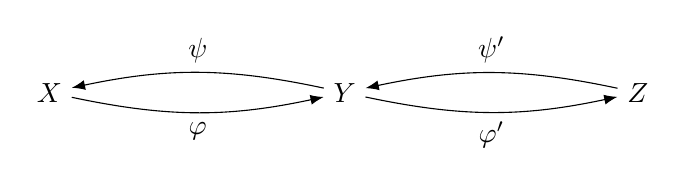
\begin{tikzpicture}[>=Latex, node distance=3.2cm]
        \node (X) {$X$};
        \node (Y) [right=of X] {$Y$};
        \node (Z) [right=of Y] {$Z$};

        % forward maps
        \draw[->] (X) to[bend right=12] node[below] {$\varphi$} (Y);
        \draw[->] (Y) to[bend right=12] node[below] {$\varphi'$} (Z);

        % backward maps (drawn slightly below)
        \draw[->] (Y) to[bend right=12] node[above] {$\psi$} (X);
        \draw[->] (Z) to[bend right=12] node[above] {$\psi'$} (Y);
        \end{tikzpicture}
        \]
        Then 
        $$\varphi' \circ \varphi \colon X \to Z, \quad \psi \circ \psi' \colon Z \to X$$
        s.t 
        \begin{align*}
            \psi \circ \psi' \circ \varphi' \circ \varphi &\sim \psi \circ \mathbbm{1} \circ \varphi \\
            &\sim \mathbbm{1}
        \end{align*}
    \end{itemize}
\end{proof}

\paragraph{Terminology.} If $X \sim \set{\cdot}$, then we say that $X$ is contractible. 
\begin{example}
    $\R^n$ is contractible; there is only one map $\varphi \colon \R^n \to \set{\cdot}$. Take the map $\psi \colon \cdot \to \R^n$ to be
    $$\cdot \to 0$$
    Indeed 
    $$\varphi \circ \psi \colon \cdot \to \cdot = \1$$

    Moreover, $\psi \circ \varphi \colon \R^n \to \R^n$ 
    $$\psi \circ \varphi (\alpha) = 0$$
    let $H \colon \R^n \times i \to \R^n$ defined by 
    $$H(x, t) = t \cdot x$$
    Similarly, we get that any convex subset of $\R^n$ is contractible; any star-shaped set is also contractible.

    Later on we will see that $S^n$ is not contractible. 
\end{example}

\begin{definition}
    Let $X$ be a space and $A \subseteq X$, then $r \colon X \to A$ is called a \emph{retraction} iff 
    $$r_{|A} = \1_{|A}$$
    In this case we say that $A$ is a \emph{retract} of $X$.
\end{definition}


\begin{example}
    \begin{itemize}
        \item Clearly the function $r \colon \R^n \to \set{x_0}$ is a retraction.
        \item $r \colon \R^n \setminus \set{0} \to S^{n-1}, \quad x \to \frac{x}{|x|}$
    \end{itemize}
\end{example}

\begin{definition}
    $X$ a space, $A \subseteq X$: we say that $X$ deformation retracts to $A$ (or that there is a deformation retraction from $x$ to $A$) 
    (or that $A$ is a deformation retract of $X$) iff 
    \begin{itemize}
        \item There is a retraction $r \colon X \to A$. 
        \item Letting $\iota \colon A \to X$ be the inclusion map, we have 
        $$r \circ \iota = \1_{|A}$$
        and 
        $$\iota \circ r \sim \1_{|X} \text{ relative to $A$}$$
    \end{itemize}
\end{definition}

\begin{example}
    \begin{itemize}
        \item $\R^n$, convex / start shaped subsets deformation retract into a point. 
        \item $\R^n$ deformation retract into $D^n$: let $r \colon \R^n \to D^n$ be defined by 
        $$r(x) = \begin{cases}
            x \quad &\text{if } x \in D^n \\
            \frac{x}{|x|} \quad &\text{if } x \not\in D^n
        \end{cases}$$
        Let $H(x, t) = t r(x) + (1-t)x$. 
        \item $\R^n \setminus \set{0}$ deformation retracts to $S^{n-1}$: $r \colon \R^n \setminus \set{0} \to S^{n-1}$ by 
        $$r(x)  = \frac{x}{|x|}$$
        $H(x,t) = (1-t) x + t \frac{x}{|x|}$ is the homotopy. 

        There is no deformation retraction from $\R^n \setminus \set{0}$ to any point.

        \item $I \times I$ (The closed rectangle) deformation retracts to a cup Exercise. 
    \end{itemize}
\end{example}

\begin{proposition}
    If $X$ deformation retracts to $A$ and $A$ to $B$, then $X$ deformation retracts to $B$.
\end{proposition}

\begin{proof}
    Exercise.
\end{proof}

\begin{theorem}
    $X \sim Y \implies \pi_1(X) \cong \pi_1(Y)$ 
\end{theorem}

\begin{lemma}
    Let $X, Y$ topological spaces and $\varphi, \psi \colon X \to Y$ be two homotopic functions by a homotopy $H \colon X \times I \to Y$. 
    Note that $H(x_0, \cdot)$ is a path in $Y$ (denote it by $\eta$). Then the following diagram commutes:
    \[
    \begin{tikzcd}
    \pi_1(X,x_0) \arrow[r,"\psi_*"] \arrow[dr,swap,"\varphi_*"] &
    \pi_1\bigl(Y,\psi(x_0)\bigr) \arrow[d,"\beta_\eta"] \\
    & \pi_1\bigl(Y,\varphi(x_0)\bigr) 
    \end{tikzcd}
    \]
    i.e 
    $$\beta_\eta \circ \psi_* = \varphi_*$$ 
\end{lemma}

\begin{proof}[Proof of lemma]
    Let $\gamma \colon I \to X$ be a loop based at $x_0$, let 
    $$H'(s,t) = \eta_t (s) \cdot H(\gamma(s), t) \cdot \overline{\eta_t} (s)$$
    Convince yourself that the endpoints match here; therefore by the Gluing Lemma $H'$ is continuous. 
    \begin{itemize}
        \item At $t = 1$, we get 
        $$\eta \cdot \psi (\gamma) \cdot \overline{\eta}$$
        \item At $t = 0$, we get 
        $$\varphi(x_0) \cdot \varphi(\gamma) \cdot \overline{\varphi(x_0)}$$
    \end{itemize}
    So we have that 
    \begin{align*}
        \eta \cdot \psi (\gamma) \cdot \overline{\eta} &\sim \varphi(x_0) \cdot \varphi(\gamma) \overline{\varphi} (x_0) \\
        &\sim \varphi (\gamma)
    \end{align*} 
    and therefore
    \begin{align*}
        [\eta \cdot \psi (\gamma) \cdot \overline{\eta}] &= [\varphi (\gamma)]  \\
        \beta_\eta [\psi(\gamma)] &= \varphi_* ([\gamma]) \\
        \beta_\eta(\psi_*([\gamma])) &= \varphi_* ([\gamma])
    \end{align*}
    therefore 
    $$\varphi_* = \beta_\eta \circ \psi_*$$
\end{proof}

\begin{proof}[Proof of the theorem]
        \[
    \begin{tikzcd}[column sep=huge]
    (Y,y_0) \arrow[r,"\psi"] &
    (X,x_0) \arrow[r,"\varphi"] &
    (Y,y_1) \arrow[r,"\psi"] &
    (X,x_1)
    \end{tikzcd}
    \]
    we know that 
    $$\psi \circ \varphi \sim \1, \quad \varphi \circ \psi \sim \1$$
    Therefore by the lemma 
    $$(\psi \circ \varphi)_* = \beta, \quad (\varphi \circ \psi)_* = \beta'$$
    But $\beta, \beta'$ are isomorphisms, therefore we get that 
    $$\varphi_* \text{ is injective and surjective}$$
\end{proof}

\subsection{Fundamental group of all spheres} 

\begin{theorem}
    $$\pi_1(S^n) = \begin{cases}
       e \quad &\text{if } n \ge 2 \\
       \Z \quad &\text{if } n = 1 \\ 
    \end{cases}$$
\end{theorem}

\begin{proof}
    \begin{itemize}
        \item $\pi_1(S^2)$; there is a homeomorphism between $S^2 \setminus \set{N}$ and $\R^2$ ($N$ is the North pole) called the stereographic projection. 
        i.e $t \to (0,0,1) + t(x, y,z) = (tx,ty, tx + 1)$ since $1 + tz = 0 \implies t = \frac{t}{1-z}$ we get the map $\Sigma$ given by 
        $$\Sigma (x,y,z) = (\frac{x}{1-z}, \frac{y}{1-z})$$
        For the inverse map $t \to (0,0,1) + t(\alpha, \beta, -1) = (t \alpha, t \beta, 1 - t)$; on the sphere 
        $$t^2 \alpha^2 + t^2 \beta^2 + (1-t)^2 = 1 \implies t = \frac{2}{\alpha^2 + \beta^2 + 1}$$
        so its inverse is given by 
        $$\Sigma^{-1} (\frac{2}{\alpha^2 + \beta^2 + 1}, \frac{2 \beta}{\alpha^2 + \beta^2 + 1}, 1 - \frac{2}{\alpha^2 + \beta^2 + 1})$$
        TODO, do the same for $\R^n$. 

        We shall take our loops to be based at the south pole $S$. Let $\gamma \colon I \to S^2$ be such a loop. If it happens that $\gamma$ never passes through $N$; 
        $\Sigma \circ \gamma$ is a loop in $\R^2$ based at $0$. Thus $H \colon I \times I \to S^2$ given by 
        $$H(s, t) = \Sigma^{-1}\left((1-t) \Sigma \circ \gamma (s) \right)$$
        gives a homotopy between $\gamma$ and the constant loop at the south pole. 

        Now suppose that we have any loop $\gamma \colon I \to S^2$. Consider the preimage by $\gamma$ of the open Northern hemisphere, this is 
        open in $I$ since $\gamma$ is continuous; in fact it is open in $(0,1)$ (and hence an open subset of $\R$). Now any open subset of $\R$ is the union of countably many 
        disjoint open intervals. Consider now the preimage of $N$, it must be closed in $[0,1]$ and hence must be compact. Therefore since the preimage of the open Northern hemisphere 
        contains that of $N$; the preimage of $N$ is an open cover of the preimage of $N$. So it has a finite subcover. Thus there are finitely many disjoint open intervals which 
        contain the preimage of $N$. Consider one of these intervals $(a, b)$. Note that $\gamma((a,b)) \subseteq N$; since $\gamma$ is continuous we can conclude that 
        $\gamma(a), \gamma(b) \in \overline{N}$ (the closed Northern hemisphere). Note that $\gamma(a), \gamma(b)$ must be on the equator; since if they were in the Northern hemisphere we would have that 
        $a$ belongs to one of the other \emph{disjoint} intervals to $(a, b)$. Note that the closed Northern hemisphere is homeomorphic to $D^2$ by $(x, y, z) \to (x,y)$. 
        but note that $\partial D^2 = S^1$ which is path connected; since we can find some path $\eta \colon I \to S^1$ going from $\gamma(a) \to \gamma(b)$ with $\eta$ homotopic $\gamma_{|[a,b]}$. 

        Now we can write a homotopy between $\gamma$ and some loop that skips $N$; see the picture we are using the homotopy above on all $(a,b)$ like above. This is continuous by the gluing 
        lemma according to our homotopy. So $\gamma$ is homotopic to a loop that skips $N$ and so homotopic to the constant loop. 

        \item We will think of $S^1$ as 
        $$\set{z \in \C \colon |z| = 1}$$
        We will base our loops at the point $z = 1$. We define 
        $$\Phi \colon \Z \to \pi_1(S^1), \quad \Phi (n) = [e^{2 \pi i n s}]$$
        We also define 
        $$p \colon \R \to S^1, \quad p(x) = e^{2 \pi i x}$$
        Note that $[p(ns)] = \Phi(n)$. We will show that $\Phi$ is a homomorphism
        \begin{align*}
            \Phi(n) \cdot \Phi(m) &= [p(ns)] \cdot [p(ms)] \\
            &= [p(ns) \cdot p(ms)] \\
            &= [p(ns) \cdot p(n + ms)] \\
            &= [p(ns \cdot (n + ms))] \\
        \end{align*}
        Note that $ns \cdot (n + ms)$ is a path $0 \to m + n$, but $\R$ is simply connected, hence 
        $$ns \cdot (n + ms) \sim (n + m)s \implies p(ns \cdot (n + ms)) \sim p((n+m) \cdot s)$$
        Therefore 
        $$\Phi(n) \cdot \Phi(m) = [p(n+m)s] = \Phi(n+m)$$
        \textbf{Claim 1.} For any path $\gamma$ in $S^1$ starting at $1$, there is a unique path $\tilde{\gamma} \in \R$ starting at $0$, s.t 
        $$p(\tilde{\gamma}) = \gamma$$
        we say that $\tilde{\gamma}$ is the \emph{lift} of $\gamma$ starting at $0$. \\
        \textbf{Claim 2.} Suppose that $\gamma_1, \gamma_2$ are two paths in $S^1$ starting at $1$, which are homotopic. Then their lifts starting at $0$ 
        are also homotopic. \\
        \textbf{$\Phi$ is surjective.} Let $[\gamma] \in \pi_1(S^1)$, then we know that there is a unique $\tilde{\gamma}$ in $\R$ s.t 
        $$\tilde{\gamma} (0) = 0, \quad p(\tilde{\gamma}) = \gamma$$
        Especially $p(\tilde\gamma(1)) = \gamma(1) = 1$, hence 
        $$\tilde \gamma(1) = n \in \Z \implies \tilde \gamma \sim ns$$
        Therefore 
        $$p(\tilde \gamma) \sim p (ns) \implies \gamma \sim p(ns) \implies [\gamma] = [p(ns)] = \Phi(n)$$
        \textbf{$\Phi$ is injective.} Suppose that $\Phi(n) = \Phi(m)$ therefore 
        $$[p(ns)] = [p(ms)]$$
        We have that the lift of $p(ns)$ is $ns$ and the lift of $p(ms)$ is $ms$ but 
        $$p(ns) \sim p(ms) \implies ns \sim ms \implies n = m$$

        We will prove the two claims in the following setting: $\tilde X, X$ two spaces, $p \colon \tilde X \to X$ s.t 
        $\forall p \in X, \ \exists U \ni p$ open then $p^{-1}(U)$ is a disjoint union of open sets s.t each one of them (say $V$) satisfies 
        $$p_{|V} \quad \text{ is a homeomorphism onto $U$}$$
        Such a $U$ is called an elementary neighborhood or an evenly covered neighborhood. $p$ is called the projection covering map and 
        $$(\tilde X, p) \text{ is called a covering space of } X$$
        The example to take in mind here is $X = S^1$, $\tilde X = \R$ with $p$ "wrapping" $\R$ around $S^1$. Indeed consider $U_1 = S^1 \setminus \set{1}$, then 
        $p^{-1} (U_1)$ $\R \setminus \Z$;  and $U_2 = S^1 \smallsetminus \set{-1}$ then $p^{-1} (U_2)$ and $U_2 = \R \setminus (1/2 \Z)$, so $(\R, p)$ is indeed a covering space 
        of $S^1$.\\
        \textbf{Claim 3.} Suppose that $(\tilde X, p)$ is a covering space of $X$, and let $f \colon Y \times I \to X$ and suppose we have some $\tilde f \colon Y \times \set{0} \to \tilde X$ 
        s.t 
        $$p \circ \tilde f = f$$
        then $\tilde f$ can be extended \emph{uniquely} to $Y \times I$ s.t $p \circ \tilde f = f$ (draw the picture).  \\
        \textbf{Proof that claim 3 implies claim 1 and 2.} For claim 1, let $Y = \set{\cdot}$, in this case 
        $$\set{\cdot} \times I \cong I$$
        so we have that $f \colon I \to X$ and $\tilde f \colon 0 \to \tilde X$ s.t $\tilde f$ can be uniquely extended to $I$; which is precisely claim 1
        where we are given a path in $X$ and the starting point of the lift is $\tilde X$. For claim 2, take $Y = I$ and $f$ to be the homotopy between 
        the two paths in $X$; from claim 1 we can lift the homotopy at the initial time; claim 3 lifts the homotopy to $\tilde X$. By uniqueness of lifts 
        the sides of the homotopy lift to the constant paths and the top of the homotopy gives a lift of the second path starting where the lift of the first path started.   

        \textbf{Proof of claim 3.} Let $y \in Y$, $\forall t \in I$ there is an open neighborhood $O_t$ of $t$ in $I$ and an open neighborhood $N_t$ of $y$ in $Y$ s.t 
        $$f(N_t \times O_t) \subseteq \text{ an elementary neighborhood}$$ 
        $\set{y} \times I$ is compact and $\set{N_t \times O_t}_{t \in I}$ is an open cover, therefore $\exists t_1, \cdots, t_k \in I$ s.t
        $$\set{y} \times I \subseteq (N_{t_1} \times O_{t_1}) \cup \cdots \cup (N_{t_k} \times O_{t_k})$$
        Let $N = \bigcap_{i = 1}^k N_{t_i}$, and let $\delta > 0$ be the Lebesgue number of the cover $O_{t_1}, \cdots, O_{t_k}$. Therefore any closed interval of length 
        $\le \delta$ is contained in one of the $O_t$'s. Consider $N \times [0, \delta]$ we know that $f (N \times [0, \delta]) \subset U$ an elementary neighborhood.
        But $p \circ \tilde f = f$, therefore $\tilde f (N \times {0}) \subset p^{-1} (U)$, let $\tilde U$ be the "part" of $p^{-1} (U)$ which contains $\tilde f (y,0)$. Now by taking the preimage 
        of $\tilde U$ by $\tilde f$ we get some open subset of $Y$ which is also an open subset of $N$; replace $N$ with this smaller subset call it $N$. Now $p$ is a homeomorphism between 
        $\tilde U$ and $U$, so it has an inverse $p^{-1} \colon U \to \tilde U$, define 
        $$\tilde f = p^{-1} \circ f$$
        This way, we have extended $\tilde f$ to $N \times [0, \delta]$. Now do the same for $N \times [\delta, 2\delta]$ by looking at $\tilde f (N \times \set{\delta})$ and making sure that 
        it maps to only one of the preimages of the new elementary neighborhood, we shrink $N$ again and extend $\tilde f$ by letting it be $p^{-1} \circ f$.   
        
        Note that by construction we have that $p \circ \tilde f = f$, and it is continuous by the Gluing lemma. Hence we know that $\forall y \in Y$, $\exists N_y$ s.t 
        $\tilde f$ is extended continuously to include $N_y \times I$ with $p \circ \tilde f = f$. Let us show that lifts of paths are unique; indeed suppose that we 
        have $\gamma \colon I \to X$ a path in $X$, and let $\tilde \gamma_1, \ \tilde \gamma_2$ be two lifts of $\gamma$ (i.e $p \circ \tilde \gamma_1 = p \tilde \gamma_2 = \gamma$ and they both have the same start point). 
        Therefore $\exists \delta > 0$ s.t any closed interval of length $\delta$ is mapped by $\gamma$ into an elementary neighborhood. Consider the interval $[0, \delta]$, we know that 
        $$\gamma \left([0,\delta]\right) \subset \text{ an elementary neighborhood $U$}$$ 
        This implies that $\tilde \gamma_1 ([0,\delta]) \subset p^{-1}(U)$ and $\tilde \gamma_2 ([0, \delta]) \subset p^{-1} (U)$; since $[0,\delta]$ is connected, we know that 
        $$\gamma_1 ([0,\delta]), \ \gamma_2 ([0,\delta]) \subset \text{ a single $\tilde U_1, \tilde U_2$}$$
        since $\tilde \gamma_1 (0) = \tilde \gamma_2 (0)$ we get $\tilde U_1 = \tilde U_2$. But since $p \circ \tilde \gamma_1 = p \circ \tilde \gamma_2$ and 
        since $p$ is a homeomorphism, then 
        $$\tilde U_1 = \tilde U_2 \to 0$$
        Proceeding similarly, we get that $\tilde \gamma_1 = \tilde \gamma_2$. 

        Note that restricting $f$ to a line like $\set{y} \times I$ gives a path in $X$, and restricting $\tilde f$ to this line gives us a lift of this path. So if we use $\tilde f$'s coming
        from different $N_y \times I$'s, then they must coincide on the intersection because the intersection is made of lines as above. So $\tilde f$ and $\tilde f$ is unique. And $\tilde f$ is continuous 
        using the gluing lemma for open sets. 
    \end{itemize}
\end{proof}

\begin{theorem}[Fundamental theorem of Algebra]
    Let $p(z) = z^n + a_{n-1} z^{n-1} + \cdots + a_0$ then 
    $$p(z_0) = 0 \text{ for some $z_0 \in \C$}$$     
\end{theorem}

\begin{proof}
    Assume that $p(z) \ne 0$ consider 
    $$H_1(s, t) = \frac{\frac{p(tre^{2 \pi i s})}{|p(tre^{2\pi i s|})}}{\frac{p(tr)}{|p(tr)|}}$$
    Note that this gives a homotopy between the constant loop  in $S^1$ at $1$ and $\frac{\frac{p(re^{2\pi i s})}{|p(re^{2 \pi i s})|}}{\frac{p(r)}{|r|}}$. Choose $r > 0$ 
    to be s.t $r > 1$ and $r > |a_{n-1}| + \cdots + |a_0|$, then notice that if $z$ is restricted to the circle of radius $r$, we have that 
    \begin{align*}
        |z|^n &= r^n = r^{n-1} \cdot r > r^{n-1} (|a_{n-1}| + \cdots + |a_0|) \\
        &> r^{n-1} |a_{n-1}| + \cdots + r^{n-1} |a_0| \\
        &> r^{n-1} |a_{n-1}| + r^{n-2} |a_{n-2}| + \cdots + |a_0| \\
        &= |a_{n-1} z^{n-1}| + \cdots + |a_0| \\
        &\ge |a_{n-1} z^{n-1} + \cdots + a_0|
    \end{align*} 
    it follows that the following polynomials depending on $t$ never vanish on the circle of radius $r$: 
    $$q_t(z) = z^n + t(a_{n-1} z^{n-1} + \cdots + a_0)$$
    This is because for $|z| = r$ we have that 
    $$q_t(z) \ge |z^n| - |t(a_{n-1} z^{n-1} + \cdots + a_0)| > 0$$
    Now consider $H_2(s,t)$ to be 
    $$H_2(s, t) = \frac{\frac{q_t(re^{2 \pi i s})}{|q_t(re^{2\pi i s|})}}{\frac{q_t(r)}{|p(r)|}}$$
    Note that this gives a homotopy between the loop which we just created (write it out TODO); and 
    $$\frac{\frac{r^n e^{2 \pi i n s}}{r^n}}{r^n/r^n} = e^{2 \pi n s}$$
    Therefore using both $H_1$ and $H_2$ we have a homotopy between the constant loop and $e^{2 \pi i ns}$ by contradiction. 
\end{proof}

\begin{theorem}[Brouwer's fixed point]
    $f \colon D^n \to D^n$ then $f$ has a fixed point, i.e $\exists p_0 \in D^n$ s.t 
    $$f(p_0) = p_0$$    
\end{theorem}

\begin{proof}
    \begin{itemize}
        \item \textbf{Case $n=1$.} Let $f \colon D^1 \to D^1$, if $f(-1) = -1$ we are done same if $f(1) = 1$. Otherwise, we get that 
        $f(-1) > -1, \ f(1) < 1$ therefore $f(x) - x$ is $> 0$ at $-1$ and $< 0$ at $1$. Therefore by the IVT, $\exists x_0 \in (-1,1)$ s.t 
        $$f(x_0) - x_0 = 0$$
        
        \item \textbf{Case $n=2$.} Assume that $f \colon D^2 \to D^2$ s.t $f(x) \ne x$ for all $x \in D^2$. Define $g \colon D^2 \to S^1$ as follows: for every $x \in D^2$, take the line 
        from $f(x)$ to $x$ then $g(x)$ is the intersection between this line and $S^1$. Note that $g$ is continuous and it is also a retraction from $D^2 \to S^1$. Take the loop $e^{2 \pi i s}$ in $D^2$, 
        then $e^{2 \pi i s}  \sim \text{ constant}$ in $D^2$. But 
        $$g(e^{2 \pi i s}) = e^{2 \pi i s} \not\sim \text{ constant loop in $S^1$}$$
        Contradiction.

        Another way of saying this is that 
        $$g_* \colon \pi_1 (D^2) \to \pi(S^1)$$
        but $\pi_1(D^2)$ is trivial, but its image is not the identity. 
    \end{itemize}
\end{proof}

\begin{corollary}
    There is no retraction $D^2 \to S^1$.
\end{corollary}

\begin{theorem}[Borsuk-Ulam Theorem]
    Let $f \colon S^n \to \R^n$ then there $\exists \in S^n$ s.t 
    $$f(x) = f(-x)$$
\end{theorem}

\begin{proof}
    \begin{itemize}
        \item \textbf{$n=1$.} We have $f \colon S^1 \to \R$, if $f(1) = f(-1)$ we are done. Otherwise wlog assume $f(1) > f(-1)$; consider 
        $$g(x) = f(x) - f(-x)$$
        then $g$ is continuous with $g(1) > 0$ and $g(-1) < 0$ therefore  by the IVT applied to the upper hemisphere, $\exists x_0 \in S^1 \cap \set{(x,y) \mid y \ge 0}$ s.t 
        $g(x_0) = 0$.
        
        \item \textbf{$n=2$.} Suppose that $f \colon S^2 \to \R^2$ with $f(x) \ne f(-x)$ for all $x$, let $g \colon S^2 \to S^1$ be defined by 
        $$g(x) = \frac{f(x) - f(-x)}{\abs{f(x) - f(-x)}}$$
        note that $g(-x) = - g(x)$. Also wlog we are going to assume that 
        $$g(1,0,0) = 1$$
        Consider now the loop 
        $$\gamma' \colon I \to S^2, \quad \gamma'(s) = (\cos (2\pi s), \sin (2\pi s), 0)$$
        Let $\gamma \colon I \to S^1$ be $g \circ \gamma'$ we know that $\pi^1 (S^2) = e$ therefore 
        $$\gamma' \sim \text{ constant}$$
        and hence 
        $$\gamma \sim \text{ constant in $S^1$}$$
        Note that $\gamma'(s + 1/2) = - \gamma'(s)$ so it follows that $\gamma(s + 1/2) = - \gamma(s)$. Consider the lift $\tilde \gamma$ of $\gamma$ starting at $0$. 
        Then (do math), we get that 
        $$\tilde \gamma(s + 1/2) - \tilde \gamma (s) = \frac{n(s)}{2}$$   
        Where $n(s)$ is odd; but since LHS is continuous $n(s)$ must be a constant $n$. i.e 
        $$\tilde \gamma(s+1/2) = \tilde \gamma (s) + n/2$$
        Hence 
        $$\tilde \gamma(1) = \tilde \gamma(1/2) + n/2 = \tilde \gamma(0) + n = n$$
        Since $\gamma$ is homotopic to the constant, $\gamma(1) = 0$ but $n$ is odd: contradiction. 
    \end{itemize}
\end{proof}

\subsection{First Algebraic Detour}
Let $\set{G_\alpha}_{\alpha \in \mathcal{A}}$ be a collection of groups, we can make a group out of the product in two ways 
\begin{enumerate}
    \item $\bigtimes_{\alpha \in \mathcal{A}} G_\alpha$ is the set of all elements in the set theoretic product with multiplication defined pointwise. 
    \item \textbf{The weak product.} $\pi_{\alpha \in \mathcal{A}} G_\alpha$ is the subgroup of the product s.t for each element only finitely many components are 
    nontrivial.
\end{enumerate}

\begin{theorem}[Universal Property of the Weak Product of Abelian Groups]
    Suppose that we have a collection $\set{G_\alpha}$ all abelian, then $\prod_{\alpha} G_\alpha$ satisfies the following property: 
    Suppose we have homomorphisms $f_\alpha \colon G_\alpha \to A$ where $A$ is abelian then $\exists ! f \colon \prod_\alpha G_\alpha \to A$ a homeomorphism 
    s.t the following diagram commutes for every $\alpha$: 
    $$\begin{tikzcd}[row sep=3.2em, column sep=4.2em]
    G_\alpha \arrow[r, "\iota_\alpha"] \arrow[dr, swap, "f_\alpha"] & \displaystyle\prod_{\beta} G_\beta \arrow[d, "f"] \\
    & A
    \end{tikzcd}$$
    Where
    $$\iota_\alpha (g) = \set{g_\beta} = \begin{cases}
        g \quad &\text{if } \alpha = p \\
        e \quad &\text{if } \alpha \ne p
    \end{cases}$$
\end{theorem}

\begin{proof}
    Let $f \left(\set{g_\alpha}\right) = \prod_\alpha f_\alpha (g_\alpha)$. Note that this product is well defined since only finitely many $f_\alpha(g_\alpha)$'s are nontrivial. 
    Moreover, the order is irrelevant since $A$ is Abelian. Clearly we have that $f$ satisfies the diagram. We also have 
    $$f(\set{g_\alpha} \set{h_\alpha}) = f(\set{g_\alpha h_\alpha}) = \prod_\alpha f_\alpha(g_\alpha h_\alpha) = \prod f_\alpha (g_\alpha) \prod f(h_\alpha)$$
    Where the last step is justified since $A$ is abelian.  

    Note that $\prod_\alpha G_\alpha$ is generated by the $i_\alpha (G_\alpha)$'s, but note that any $f'$ that satisfies the diagram must agree with our $f$ on each of 
    these $G_\alpha$'s (both  give us $f_\alpha (G_\alpha)$) therefore $f' = f$. 
\end{proof}

\begin{remark}
    Note that the universal property of the weak product defines it (up to isomorphism). Indeed,
    suppose that we have a collection $\set{G_\alpha}$ all abelian, and some abelian $G$ that satisfies the following property: 
    For any $A$ and any homomorphisms $f_\alpha \colon G_\alpha \to A$ and homomorphisms $\iota_\alpha \colon G_\alpha \to G$
    where $A$ is abelian and $\exists ! f \colon G\to A$ a homomorphism 
    s.t the following diagram commutes for every $\alpha$: 
    $$\begin{tikzcd}[row sep=3.2em, column sep=4.2em]
    G_\alpha \arrow[r, "\iota_\alpha"] \arrow[dr, swap, "f_\alpha"] & \displaystyle G\arrow[d, "f"] \\
    & A
    \end{tikzcd}$$
    Then $G \cong \prod_{\alpha \in \mathcal{A}} G_\alpha$.
\end{remark}

\begin{proof}
    Draw the commutative diagram. 
\end{proof}

\begin{definition}
Let $S$ be a set. The \emph{free abelian group on $S$} is an abelian group $F(S)$ together with a map
\[
\iota \colon S \to F(S)
\]
such that for every abelian group $A$ and every map $\chi \colon S \to A$ there exists a unique group homomorphism
\[
\varphi \colon F(S) \to A
\]
making the following diagram commute:
\[
\begin{tikzcd}
S \arrow[r, "\iota"] \arrow[dr, "\chi"'] & F(S) \arrow[d, "\varphi"] \\
& A
\end{tikzcd}
\]
\end{definition}


\begin{example}
    Let $S = \set{x}$, let $F(S) = \Z$ and $j \colon \set{x} \to \Z$ be defined by $j(x) = 1$. Pick any $A$ abelian, let $\chi \colon S \to A$ let 
    $a = \chi(x)$ an define 
    $$\varphi \colon \Z \to A, \quad \varphi(n) = a^n$$
    indeed, $\varphi(j(x)) = a = \chi (x)$ abd $\varphi$ is unique since it $\varphi'(1) = a$ and $1$ generates $\Z$. 

    Generally we write elements of $F(\set{x})$ as $nx$. 
\end{example}

\begin{theorem}
    The free abelian group of $S$ is unique up to isomorphism. 
\end{theorem}

\begin{proof}
    Draw the picture; final element is unique.
\end{proof}

\begin{theorem}
    Suppose that $S = \bigcup_{\alpha \in \mathcal{A}} S_\alpha$ with $\alpha \ne \alpha' \implies S_\alpha \cap S_\alpha' = \varnothing$, then 
    $$F(S) \cong \prod_\alpha F(S_\alpha)$$
\end{theorem}

\begin{proof}
\[
\begin{tikzcd}[row sep=3.2em, column sep=4.2em]
S_\alpha
  \arrow[r,"j_{S_\alpha}"]
  \arrow[d,hookrightarrow,"i_\alpha"']
&
F(S_\alpha)
  \arrow[r,"\iota_\alpha"]
  \arrow[d,"\varphi_\alpha"']
&
\displaystyle \prod_{\beta\in\mathcal A} F(S_\beta)
  \arrow[d,dashed,"\Phi"]
\\
S
  \arrow[r,"j_S"']
  \arrow[rr,bend right=18,"\chi"']
&
F(S)
  \arrow[r,"\overline{\chi}"']
&
A
\end{tikzcd}
\]
\end{proof}

\begin{corollary}
    For any $S$, note that 
    $$F(S) \cong \prod_{x \in S} F(\set{x}) \cong \prod_{x \in S} \Z$$
    We write elements in $F(S)$ as 
    $$n_1 x_1 + \cdots + n_k x_k$$
    This notation is useful because multiplication in $F(S)$ corresponds to addition of coefficients.
\end{corollary}

\begin{theorem}
    Any abelian group $A$ is the homomorphic image of a free abelian group. 
\end{theorem}

\begin{proof}
    Let $S = A$ and let $\chi \colon S \to A = \1$; draw the diagram the proof is done.     
\end{proof}

\begin{example}
    Let $\Z_2 $, take $A = \Z_2$ and find the $\varphi \colon F(A) \to A$. But also let $\varphi \colon \Z \to \Z_2$ defined by 
    $$\varphi (n) = n \mod 2$$
\end{example}

\begin{definition}
    let $A$ be an abelian group suppose that $F(S)$ is free abelian on $S$ and 
    $$\varphi \colon F(S) \to A \quad \text{surjective}$$
    Every nontrivial element of the kernel of $\varphi$ is said to be a non-trivial relation on the generators of $A$. 
    Moreover if $r_1, \cdots, r_k$ are nontrivial relation and $r_{k+1} \in \angles{r_1, \cdots, r_k}$, then we say that 
    $r_{k+1}$ is a consequence of $r_1, \cdots, r_k$. If $r_1, \cdots, r_k$ generate the whole kernel, we say that we have a presentation 
    of $A$ in terms of generators and relations. 
\end{definition}

\begin{example}
    In the example above write $\Z = F(\set{x})$, think of $A$ as being generated by $x$ with the following relations imposed: 
    $$x + x = 0, \quad x + x + x + x = 0, \quad -x-x = 0, \cdots$$
    Note that $x + x + x + x$ is a consequence of $x + x$. Indeed, since all relations are a consequence of $x + x = 0$, therefore 
    $\Z_2$ is generated by a single element with a single relation.  
\end{example}

%%%%%%%%%%%%%%%%%%%%%%%%%%%%%%%%%%%%%%%%%%%%%%%%%%%%%%%%%%%%%%%%%%%%%%
% Free Groups and Free Products — Cleaned Lecture Notes
%%%%%%%%%%%%%%%%%%%%%%%%%%%%%%%%%%%%%%%%%%%%%%%%%%%%%%%%%%%%%%%%%%%%%%

%%%%%%%%%%%%%%%%%%%%%%%%%%%%%%%%%%%%%%%%%%%%%%%%%%%%%%%%%%%%%%%%%%%%%%
\subsection*{Free Groups}
%%%%%%%%%%%%%%%%%%%%%%%%%%%%%%%%%%%%%%%%%%%%%%%%%%%%%%%%%%%%%%%%%%%%%%

\begin{definition}[Free group]
Let $S$ be a set. A \emph{free group} on $S$, denoted $F^*(S)$ (often written $F(S)$),
is a group together with a function
\[
j : S \to F^*(S)
\]
such that for every group $G$ and every function
\[
\chi : S \to G
\]
there exists a unique group homomorphism
\[
\varphi : F^*(S) \to G
\]
making the following diagram commute:
\[
\begin{tikzcd}
S \arrow[r,"j"] \arrow[dr,"\chi"'] & F^*(S) \arrow[d,"\varphi"] \\
& G
\end{tikzcd}
\]
i.e. $\varphi \circ j = \chi$.

Equivalently, $(F^*(S),j)$ is the initial object in the category of
groups equipped with a map from $S$.
\end{definition}

\begin{theorem}[Uniqueness]
The free group on $S$ is unique up to isomorphism.
\end{theorem}

\begin{proof}
Let $(F_1,j_1)$ and $(F_2,j_2)$ be two free groups on $S$.
By the universal property, there exist unique homomorphisms
\[
\phi : F_1 \to F_2, \qquad \psi : F_2 \to F_1
\]
such that $\phi \circ j_1 = j_2$ and $\psi \circ j_2 = j_1$.
Then $\psi\circ\phi : F_1 \to F_1$ is a homomorphism satisfying
$(\psi\circ\phi)\circ j_1 = j_1$.
By uniqueness it must be the identity, hence $\psi\circ\phi = \mathrm{id}$.
Similarly $\phi\circ\psi = \mathrm{id}$, so $F_1 \cong F_2$.
\end{proof}

\begin{example}
If $S=\{x\}$ then $F^*(S)\cong \mathbb Z$.
\end{example}

\begin{proof}
Define $j(x)=1\in \mathbb Z$. Given any group $G$ and map $\chi:S\to G$,
write $\chi(x)=g$. Define
\[
\varphi:\mathbb Z \to G, \qquad \varphi(n)=g^n.
\]
This is the unique homomorphism with $\varphi\circ j=\chi$, hence
$\mathbb Z$ satisfies the universal mapping property.
\end{proof}

%%%%%%%%%%%%%%%%%%%%%%%%%%%%%%%%%%%%%%%%%%%%%%%%%%%%%%%%%%%%%%%%%%%%%%
\subsection*{Free Products}
%%%%%%%%%%%%%%%%%%%%%%%%%%%%%%%%%%%%%%%%%%%%%%%%%%%%%%%%%%%%%%%%%%%%%%

\begin{definition}[Free product]
Let $\{G_\alpha\}_{\alpha\in\mathcal A}$ be a family of groups.
The \emph{free product}
\[
\prod_{\alpha\in\mathcal A}^{*} G_\alpha
\]
is a group together with homomorphisms
\[
i_\alpha : G_\alpha \to \prod_{\alpha}^{*} G_\alpha
\]
such that for any group $G$ and any family of homomorphisms
\[
f_\alpha : G_\alpha \to G
\]
there exists a unique homomorphism
\[
f : \prod_{\alpha}^{*} G_\alpha \to G
\]
making the diagrams commute:
\[
\begin{tikzcd}
G_\alpha \arrow[r,"i_\alpha"] \arrow[dr,"f_\alpha"'] &
\prod_{\alpha}^{*} G_\alpha \arrow[d,"f"] \\
& G
\end{tikzcd}
\]
i.e. $f\circ i_\alpha = f_\alpha$ for all $\alpha$.
\end{definition}

%%%%%%%%%%%%%%%%%%%%%%%%%%%%%%%%%%%%%%%%%%%%%%%%%%%%%%%%%%%%%%%%%%%%%%
\subsection*{Free Groups as Free Products}
%%%%%%%%%%%%%%%%%%%%%%%%%%%%%%%%%%%%%%%%%%%%%%%%%%%%%%%%%%%%%%%%%%%%%%

\begin{theorem}
Suppose $S=\bigsqcup_\alpha S_\alpha$ is a disjoint union of sets.
Then
\[
F^*(S) \cong \prod_{\alpha}^{*} F^*(S_\alpha).
\]
\end{theorem}

\begin{proof}
Both sides satisfy the same universal mapping property for maps from $S$.
Hence they are isomorphic by uniqueness of universal objects.
\end{proof}

\begin{corollary}
Let $S$ be any set. Then
\[
F^*(S) \cong \prod_{s\in S}^{*} F^*(\{s\})
\cong \prod_{s\in S}^{*} \mathbb Z.
\]
\end{corollary}

\begin{corollary}
Every group is a homomorphic image of a free group.
\end{corollary}

\begin{proof}
Let $G$ be a group and take $S=G$ as a set.
The identity map $S\to G$ extends uniquely to a homomorphism
\[
F^*(S)\to G
\]
which is surjective.
\end{proof}

%%%%%%%%%%%%%%%%%%%%%%%%%%%%%%%%%%%%%%%%%%%%%%%%%%%%%%%%%%%%%%%%%%%%%%
\subsection*{Generators and Relations}
%%%%%%%%%%%%%%%%%%%%%%%%%%%%%%%%%%%%%%%%%%%%%%%%%%%%%%%%%%%%%%%%%%%%%%

\begin{definition}
Let $G$ be a group and suppose
\[
f : F^*(S) \twoheadrightarrow G
\]
is a surjective homomorphism.

\begin{itemize}
\item The elements of $S$ (via their images in $G$) are called
generators.
\item The nontrivial elements of $\ker(f)$ are called relations.
\item If $r_1,\dots,r_k\in F^*(S)$ then $r_{k+1}$ is a consequence
of them if
\[
r_{k+1}\in \langle\!\langle r_1,\dots,r_k\rangle\!\rangle,
\]
the smallest normal subgroup containing $r_1,\dots,r_k$.
\end{itemize}
\end{definition}

%%%%%%%%%%%%%%%%%%%%%%%%%%%%%%%%%%%%%%%%%%%%%%%%%%%%%%%%%%%%%%%%%%%%%%
\subsection*{Existence of Free Products}
%%%%%%%%%%%%%%%%%%%%%%%%%%%%%%%%%%%%%%%%%%%%%%%%%%%%%%%%%%%%%%%%%%%%%%

\begin{theorem}
Free products exist.
\end{theorem}

\begin{proof}[Construction via reduced words]

Let $\mathcal A=\bigsqcup_\alpha G_\alpha$ be the disjoint union
of the underlying sets.

\paragraph{Words.}
A word is a finite sequence
\[
w=g_1 g_2 \cdots g_n
\quad \text{with } g_i\in G_{\alpha_i}.
\]

A word is \emph{reduced} if:

\begin{enumerate}
\item $g_i \neq e$ for all $i$,
\item adjacent letters come from different groups:
      $\alpha_i \neq \alpha_{i+1}$.
\end{enumerate}

The empty word is denoted by $e$.

\paragraph{Multiplication.}
Define multiplication by:

\begin{itemize}
\item concatenation of words,
\item followed by reduction:
      \begin{itemize}
      \item multiply adjacent elements from the same group,
      \item remove identities,
      \item cancel inverse pairs.
      \end{itemize}
\end{itemize}

\paragraph{Group axioms.}

\begin{itemize}
\item Identity: the empty word.
\item Inverse:
\[
(g_1\cdots g_n)^{-1}=g_n^{-1}\cdots g_1^{-1}.
\]
\item \textbf{Associativity.}
    Let $W$ denote the set of reduced words. For each letter $g$ (i.e.\ an element
    of some $G_\alpha$), define the map
    \[
    L_g : W \to W, \qquad L_g(w) = g \cdot w,
    \]
    where the product on the right means concatenation followed by reduction.

    Let $w = h_1 \cdots h_n$ be a reduced word. Then
    \[
    L_{g^{-1}} \circ L_g (h_1 \cdots h_n)
    = L_{g^{-1}}(g h_1 \cdots h_n).
    \]
    We consider cases:

    \begin{itemize}
    \item If $g$ and $h_1$ belong to different groups, no reduction occurs,
    and
    \[
    L_{g^{-1}}(g h_1 \cdots h_n)
    = h_1 \cdots h_n.
    \]

    \item If $g$ and $h_1$ belong to the same group, two subcases arise:
    \begin{itemize}
    \item If $h_1 \neq g^{-1}$, then multiplication inside the group replaces
    $g h_1$ by a single element, and applying $L_{g^{-1}}$ restores
    $h_1 \cdots h_n$ after reduction.

    \item If $h_1 = g^{-1}$, cancellation occurs and
    \[
    L_{g^{-1}}(g h_1 \cdots h_n)
    = g^{-1} h_2 \cdots h_n
    = h_1 h_2 \cdots h_n.
    \]
    \end{itemize}
    \end{itemize}

    Hence $L_{g^{-1}} \circ L_g = \mathrm{id}$, so $L_g$ is a bijection
    with inverse $L_{g^{-1}}$.

    Now let $w = g_1 \cdots g_n$ be a reduced word and define
    \[
    L_w := L_{g_1} \circ \cdots \circ L_{g_n}.
    \]
    Then $L_w$ is a bijection as a composition of bijections.

    Moreover, the map
    \[
    w \longmapsto L_w
    \]
    is injective. Indeed, if $w_1 \neq w_2$, then
    \[
    L_{w_1}(e) = w_1 \neq w_2 = L_{w_2}(e),
    \]
    where $e$ denotes the empty word.

    Suppose
    \[
    w_1 = g_1 \cdots g_n h_1 \cdots h_m,
    \qquad
    w_2 = h_m^{-1} \cdots h_1^{-1} k_1 \cdots k_\ell,
    \]
    so that reduction gives
    \[
    w_1 \cdot w_2 = g_1 \cdots g_n k_1 \cdots k_\ell.
    \]
    Then
    \[
    L_{w_1 \cdot w_2}
    = L_{g_1} \circ \cdots \circ L_{g_n}
    \circ L_{k_1} \circ \cdots \circ L_{k_\ell}.
    \]
    On the other hand,
    \[
    L_{w_1} \circ L_{w_2}
    = L_{g_1} \circ \cdots \circ L_{g_n}
    \circ L_{h_1} \circ \cdots \circ L_{h_m}
    \circ L_{h_m^{-1}} \circ \cdots \circ L_{h_1^{-1}}
    \circ L_{k_1} \circ \cdots \circ L_{k_\ell},
    \]
    and the middle terms cancel since
    $L_{h_i} \circ L_{h_i^{-1}} = \mathrm{id}$.
    Thus
    \[
    L_{w_1} \circ L_{w_2} = L_{w_1 \cdot w_2}.
    \]

    Finally,
    \[
    L_{(w_1 \cdot w_2)\cdot w_3}
    = (L_{w_1}\circ L_{w_2})\circ L_{w_3}
    = L_{w_1}\circ (L_{w_2}\circ L_{w_3})
    = L_{w_1 \cdot (w_2 \cdot w_3)}.
    \]
    Since the map $w \mapsto L_w$ is injective, we conclude
    \[
    (w_1 \cdot w_2)\cdot w_3
    = w_1 \cdot (w_2 \cdot w_3),
    \]
    establishing associativity.
\end{itemize}

We still need to show that this group respects the UMP of the Free product. Indeed, we define 
$$i_\alpha \colon G_\alpha \to W, \quad i_\alpha(g) = g$$
This is a valid homomorphism since 
$$i_\alpha (g \cdot h) = (gh) = g \cdot h = i_{\alpha} (g) \cdot i_\alpha (h)$$
Suppose that we have $G$ and 
$$f_\alpha \colon G_\alpha \to G$$
Let $f \colon w \to G$ be defined as follows: 
$$f(g_1 \cdots g_n) = f_{\alpha_1}(g_1) f_{\alpha_2}(g_2) \cdots f_{\alpha_n} (g_n)$$
Note that $f$ does make the diagram commute, take $g \in G_\alpha$ we get
$$f_\alpha(g) = f(i_\alpha(g))$$
We still need to show that it is a homomorphism, let $w = g_1 \cdots g_n h_1 \cdots h_m$ and $w_2 = h_m^{-1} \cdots h_1^{-1} k_1 \cdots k_l$
s.t $w_1 \cdot w_2 = g_1 \cdots g_n k_1 \cdots k_l$  then 
\begin{align*}
    f(w_1) f(w_2) &= f_{\alpha_1} (g_1) \cdots f_{\alpha_n} (g_n) f_{\beta_1}(h_1) \cdots f_{\beta_m} (h_m) f_{\beta_m} (h_m^{-1}) \cdots f_{\beta_1}(h_1) f_{\gamma_1} (k_1) \cdots f_{\gamma_l} (k_l) \\
    &= f(w_1 \cdot w_2)
\end{align*} 
Note that any homomorphism that makes the diagram commute must agree with $f$ on the one letter words, which generate the product. Therefore $f$ is indeed unique. 
\end{proof}

\section{The Van Kampen Theorem}
Let $X$ be a space with 
$$X = \bigcup_{\alpha \in \mathcal{A}} A_\alpha, \quad \bigcap_{\alpha \in \mathcal{A}} A_\alpha \ne \varnothing$$
Fix $x_0 \in \bigcap_{\alpha \in \mathcal{A}} A_\alpha$, therefore all the fundamental groups below will be based at $x_0$. Let $\iota_\alpha \colon A_\alpha \to X$ 
be the usual inclusion map. So we get 
$$\iota_\alpha^* \colon \pi_1 (A_\alpha) \to \pi_(X)$$
Thus we get a unique homomorphism 
$$\Phi \colon \prod_{\alpha \in \mathcal{A}}^* \pi_1(A_\alpha) \to \pi_1(X)$$
such that the following diagram commutes: 
\[
\begin{tikzcd}
\pi_1(A_\alpha,x_0) \arrow[r,"i_\alpha"] \arrow[dr,swap,"\iota_{\alpha}"] &
{\displaystyle \prod^\ast_{\beta\in\mathcal A}\,\pi_1(A_\beta,x_0)} \arrow[d,"\Phi"] \\
& \pi_1(X,x_0)
\end{tikzcd}
\]

\begin{theorem}[The Van Kampen Theorem]
    Suppose we have the setting above, and $A_\alpha$'s are open, $A_\alpha \cap A_\beta$ is path connected, $A_\alpha \cap A_\beta \cap A_\gamma$ is path connected. 
    Then $\Phi \colon \prod_{\alpha} \pi_1(A_\alpha) \to \pi_1(X)$ is surjective and
    $\ker \Phi$ is the smallest normal subgroup generated by elements of the form 
    $$\left[i_\alpha \left(\iota_{\alpha \beta}^* ([\gamma])  \right)\right]^{-1} \left[i_\beta \left(\iota_{\beta \alpha}^* ([\gamma])\right)\right]$$
    Where 
    $$[\gamma] \in \pi_1(A_\alpha \cap A_\beta)$$
    and 
    $$\iota_{\alpha \beta} \colon A_\alpha \cap A_\beta \to A_\alpha \quad \text{inclusion}$$
\end{theorem}

\begin{remark}
    Note that 
    \begin{align*}
        \Phi \left[i_\alpha \left(\iota_{\alpha \beta}^* ([\gamma])  \right)\right] &= \iota^*_\beta \left(\iota_{\beta \alpha}^* ([\gamma])\right) \\
        &= (\iota_\beta \circ \iota_{\beta \alpha})^* (\gamma)
    \end{align*}
    Similarly 
    \begin{align*}
        \Phi \left[i_\beta \left(\iota_{\beta \alpha}^* ([\gamma])\right)\right] &= \iota_\alpha^* (\iota_{\alpha\beta}^* ([\gamma])) \\
        &= (\iota_{\alpha} \circ \iota_{\alpha \beta})^* [\gamma]
    \end{align*}
    Since $\iota_\beta \circ \iota_{\beta \alpha} = \iota_\alpha \circ \iota_{\alpha \beta}$ we have 
    $$(\iota_\beta \circ \iota_{\beta \alpha})^* = (\iota_\alpha \circ \iota_{\alpha \beta})^*$$ 
    So a priori we have that if $H$ Is the smallest normal subgroup generated by these, we have that (in general)
    $$H \subset \ker \Phi$$
    The theorem gives us 
    $$\ker \phi = H$$
\end{remark}

We will now demonstrate that all the conditions above are necessary: 
\begin{example}[Double intersection]
    Take $S_1$ as the open union of two arcs (more than half-arcs). Note that their intersection is not path connected. Well 
    $$\pi_1(S_1) = \Z, \ \pi_1(P_1) = \pi_1(P_2) = e$$ 
\end{example}

\begin{example}[Triple intersection]
    View picture, lots of drawing. 
\end{example}

\begin{example}[$A_\alpha$ open]
    Hawaiian earrings; i.e take circles of radius $1/n$ centered at $(1/n,0)$. Let $A_\alpha$'s be the circles, if SVK applies, then 
    the fundamental group would be 
    $$\prod_{\text{circles}}^* \Z$$
    This would imply that any loop in this space is homotopic to a loop contained in finitely many circles. However, it is easy to see 
    that this is not the case (we will show this in an assignment).
\end{example}

\begin{proof}
    To show surjectivity, we need to show that for any loop $\gamma \in X$ we can find finitely many loops $\gamma_1, \cdots, \gamma_n$ each one in some $A_{\alpha_i}$. Such that 
    $\gamma \sim \gamma_1 \cdots \gamma_n$. Since the $A_\alpha$'s are open, we have that 
    $\gamma^{-1} (A_\alpha)$ is open in $I$. Therefore 
    $$\set{\gamma^{-1} (A_\alpha)}_{\alpha \in \mathcal{A}} \text{ is an open cover of $I$}$$
    Let $\delta > 0$ be a Lebesgue number of this cover, i.e any closed interval of length $\delta$ is contained in some $\gamma^{-1} (A_\alpha)$. 
    i.e for any closed interval of length $\delta$, its image by $\gamma$ is contained in some $A_\alpha$. We are going to use the fact that if the domain 
    of a path is decomposed into intervals, then the original path is homotopic to the product of the paths obtained by restricting the original path to these intervals.
    In our case, we get that $\gamma \sim \gamma_1 \cdot \gamma_2 \cdots \gamma_n$, where each $\gamma_i$ is contained in some $A_{\alpha_i}$. Let $x_i = \gamma_i(1)$, 
    since $A_\alpha \cap A_\beta$ is path connected, we can take some path $\eta_i$ from $x_0 \to x_i$ contained in $A_{\alpha_i} \cap A_{\alpha_{i+1}}$. 
    Notice that 
    $$\gamma \sim (\gamma_1 \cdot \overline{\eta}_1) \cdot (\eta_1 \cdot \gamma_2 \cdot \overline{\eta_2}) \cdots (\gamma_{n-1} \cdot \gamma_n)$$
    Where the $(\bullet)$ are loops in the $A_\alpha$'s. Now by combining adjacent loops which live in the same $A_\alpha$'s and removing those that are nullhomotopic 
    in $A_\alpha$, we get what we want. 
    
    To show that the kernel of $\Phi$ is $N$ (the normal subgroup described in the theorem), it is enough to show that 
    $$\Phi (w_1) = \Phi(w_2) \implies w_2^{-1} w_1 \in N$$
    Let $w_1 \in K$ and $w_2 = e$ therefore 
    $$\Phi(e) = \Phi (w_1)$$
    hence $e w_1 \in N$. 

    Given a loop $\gamma$ in $X$, a factorization of $\gamma$ is a not necessarily reduced word from the alphabet $\bigcup_{\alpha \in \mathcal{A}} \pi_1(A_\alpha)$, i.e a finite string 
    of the form 
    $$[\gamma_1] [\gamma_2] \cdots [\gamma_n], \quad [\gamma_i] \in \pi_1(A_{\alpha_i})$$ 
    such that 
    $$\gamma \sim \gamma_1 \cdot \gamma_2 \cdots \gamma_n$$
    by the surjectivity above, we get that every loop has a factorization. 

    Moreover, we say that two factorization of any loop are equivalent if they can be related by a finite sequence of the following operations: 
    \begin{enumerate}
        \item Adding or removing identities. 
        \item combining or splitting adjacent letters if they come from the same group. 
        \item $$[\gamma_1] \cdots [\gamma_i]_{\alpha} \cdots [\gamma_n] \rightleftarrows [\gamma_1] \cdots [\gamma_i]_{\beta} \cdots [\gamma_n]$$
        where if $\gamma_i \in A_\alpha \cap A_\beta$, we replace $\gamma_i \in A_\alpha$ to its inclusion to $A_\beta$. i.e we are changing 
        $$\iota^*_{\alpha \beta} [\gamma_i] \rightleftarrows \iota^*_{\beta \alpha} [\gamma_i]$$  
    \end{enumerate}

    \textbf{Claim.} Two factorizations are equivalent $\implies$ the corresponding reduces words are in the same coset of $N$. \\
    \textbf{Proof of claim.} Moves $1$ and $2$ do not change the reduced words. Consider two words that are related by move $3$, therefore 
    \begin{align*}
        [\gamma_n]^{-1} \cdots [\gamma_i]_{\alpha}^{-1} \cdots [\gamma_1]^{-1} [\gamma_1] \cdots [\gamma_i]_\beta \cdots [\gamma_n] &= [\gamma_n]^{-1} \cdots [\gamma_i]_\alpha^{-1} [\gamma_i]_\beta^{-1} \cdots [\gamma_n] \\
        &= (\cdots [\gamma_n])^{-1} [\gamma_i]^{-1}_\alpha [\gamma_i]_\beta (\cdots [\gamma_n]) \in N
    \end{align*}
    (Since $[\gamma_i]^{-1}_\alpha [\gamma_i]_\beta$ is a generator of $N$, by definition). 

    So suppose that we have $w_1 = [\gamma_1] \cdots [\gamma_n], \ w_2 = [\gamma_1'] \cdots [\gamma_m']$ s.t $\Phi(w_1) = \Phi(w_2)$; i.e 
    $$[\gamma_1] \cdots [\gamma_n] \sim [\gamma_1'] \cdots [\gamma_m']$$
    So $[\gamma_1] \cdots [\gamma_n]$ and $[\gamma_1'] \cdots [\gamma_m']$ are two factorization of the same loop. Since 
    $$\gamma_1 \cdots \gamma_n \sim \gamma_1' \cdots \gamma_m'$$
    we have a homotopy 
    $$H \colon I \times I \to X$$
    Note that $\set{H^{-1} (A_\alpha)}_\alpha$ is an open cover of $I \times I$, therefore $\exists \delta > 0$ s.t any closed square of sides $\le 2 \delta$ is contained in one of
    these those sets. i.e its image by $H$ is contained in one of the $A_\alpha$'s. Take $I \times I$, divide it into squares of size $\le \delta \times \delta$ wlog 
    we can assume that the endpoints of the $\gamma$'s are in the grid already.

    By construction associate to each of the rectangles and $A_\alpha$ to which it goes by $H$. By moving the vertical edges of every other row, we can make sure 
    that at no point is shared by more than three rectangles, note that not to move the first and last make sure that we have odd number of rows. Now for every corner 
    of every rectangle, we take a path from $x_0$ to the image of that corner by $H$ in the intersection of the $A_\alpha$'s sharing that corner. For the points on the 
    lowest and highest edges, also require that these paths are in $A_\alpha$'s in which the corresponding $\gamma_i$' lives. 

    Note that any line that goes from left to right, gives  a loop by restricting $H$ to this line. Note that we can associate to this loop several 
    factorizations by inserting $\overline{\eta} \eta$ at every corner. View the picture. 

    \textbf{Claim.} All these factorizations are equivalent and are equivalent to $\gamma_1 \cdots \gamma_n$ and $\gamma_1' \cdots \gamma_m'$. \\
    \textbf{Subclaim 1.} All factorizations corresponding to the same line are equivalent. This is clear since the different choices of $A_\alpha$'s correspond 
    exactly to move $3$. \\
    \textbf{Subclaim 2.} The factorizations corresponding to the bottom / top edges are equivalent to $\gamma_1 \cdots \gamma_n$ / $\gamma_1' \cdots \gamma_n'$. By applying 
    move $3$ at every edge if needed. We make sure that the edges making up $\gamma_i$ are in the $A_\alpha$ corresponding to it. Then apply move $2$ to combine the loops into 
    $\gamma$'s (or $\gamma$'s). \\
    \textbf{Subclaim 3.} Two lines that differ by a square (picture blue and red) give equivalent factorizations. By subclaim 1, we pick the factorizations that 
    coincide everywhere away from the square; Moreover, for those on the square we choose the $A_\alpha$ which correspond to that rectangle. However, the loops corresponding to 
    these two are homotopic. This is because the image of two homotopic paths under a continuous function are homotopic. 
    
    This proves the claim, and hence the theorem.
\end{proof}

\begin{corollary}
    $\pi_1 (S^n) = e$ for $n \ge 2$.
\end{corollary}

\begin{proof}
    Cut the sphere into two $2/3$-spheres. Note that both $2/3$-spheres ($S_1, S_2$) are homeomorphic to a disk (which is nullhomotopic), therefore By VK 
    $$\pi_1 (S) = \frac{\pi_1(S_1) \star \pi_1(S_2)}{N} \cong e$$
\end{proof}



\end{document}